\chapter{電子状態の計算}
\begin{summary}
第一原理計算は、物質中の電子の波動関数を密度半関数法を用いて計算している。この計算には、自己無撞着計算が必要であり、反復計算を行うことで十分に収束した波動関数が得られる。得られた波動関数は、電子状態密度やバンド分散など、さまざまな電子状態の物理量を計算するために使用することができる。この章では、自己無撞着計算やその結果を利用した電子状態密度やバンド分散の計算方法を説明する。
\end{summary}

\newpage

\section{自己無撞着計算}
自己無撞着計算(Self-consistent Field, SCF)計算を行うための入力ファイルを作成する。
GaNのSCF計算の入力ファイルは下記のとおりである。
入力ファイルの作成、計算結果の確認は文献\cite{maezono_DFT}を参考におこなった。

\begin{example}{GaN.scf.in}
\begin{verbatim}
  &control
    calculation = 'scf'
    restart_mode = 'from_scratch'
    prefix = 'gan'
    outdir = 'out_gan'
    pseudo_dir = './PP'
  /
  &system
    ibrav = 4
    a = 3.2153
    c = 5.23899
    nat = 4
    ntyp = 2
    occupations = 'fixed'
    ecutwfc = 50
    ecutrho = 400
    nbnd = 20 !18 filled bands, 2 more empty bands
  /
  &electrons
  /
  K_POINTS {automatic}
  2 2 2 1 1 1
  ATOMIC_SPECIES
    Ga   69.72300  Ga.pbe-dn-kjpaw_psl.1.0.0.UPF
     N   14.00650  N.pbe-n-kjpaw_psl.1.0.0.UPF
  ATOMIC_POSITIONS {crystal}
  Ga 0.6666680851 0.3333319134 0.0000000000
  Ga 0.3333319519 0.6666680855 0.5000260061
  N  0.6666925477 0.3333074525 0.3766951515
  N  0.3333074513 0.6666925484 0.8767004581
\end{verbatim}
\end{example}
原子位置は第2章で計算した構造最適化の結果を利用している。

自己無撞着計算が終わったら、正しく計算が行われているのか確認する。
計算結果であるscf.outからtotal energyの項を次のようなコマンドで確認する。
\begin{code}
\begin{verbatim}
  grep 'total energy ' scf.out
\end{verbatim}
\end{code}
上記のコマンドを実行すると下記のようにtotal energyの値が表示される。
\begin{code}
\begin{verbatim}
  total energy              =    -611.70547437 Ry
  total energy              =    -612.17226092 Ry
  total energy              =    -612.41317647 Ry
  ...
  total energy              =    -612.45360188 Ry
  total energy              =    -612.45360152 Ry
! total energy              =    -612.45360151 Ry
\end{verbatim}
\end{code}
自己無撞着計算のイタレーションの過程におけるtotal energyが表示されており、次第に収束していっていることが確認できる。
エネルギーが十分に収束していなくても、イタレーション回数の上限に達すると計算が終了するため、まずは収束しているかどうかを確認することが重要である。
計算が収束していることを確認出来たら、次は状態密度の計算を行う。
\section{状態密度の計算}
状態密度の計算は先ほど自己無撞着計算で得られた電子状態を用いて行う。ここでは、自己矛盾な状態に十分収束した結果を使うので、SCFループを回す必要はない。
収束し終えた結果を使って計算することから、non-SCFという意味で、NSCF計算と呼ぶ。

\subsection{NSCF計算}
先ほどのGaNのSCF計算に使用したインプットファイルをコピーして、NSCF計算用に次のように書き換える。
\begin{example}{GaN.nscf.dos.in}
\begin{verbatim}
  &control
  calculation = 'nscf'
  restart_mode = 'from_scratch'
  prefix = 'gan'
  outdir = 'out_gan'
  pseudo_dir = './PP'
/
&system
  ibrav = 4
  a = 3.21374
  c = 5.23521
  nat = 4
  ntyp = 2
  occupations = 'tetrahedra'
  ecutwfc = 50
  ecutrho = 400
  nbnd = 20 ! 18 filled bands , 2 more empty bands
/
&electrons
/
K_POINTS {automatic}
4 4 2 0 0 0
ATOMIC_SPECIES
  Ga   69.72300  Ga.pbe-dn-kjpaw_psl.1.0.0.UPF
   N   14.00650  N.pbe-n-kjpaw_psl.1.0.0.UPF
   ATOMIC_POSITIONS {crystal}
   Ga 0.6666680851 0.3333319134 0.0000000000
   Ga 0.3333319519 0.6666680855 0.5000260061
   N  0.6666925477 0.3333074525 0.3766951515
   N  0.3333074513 0.6666925484 0.8767004581
\end{verbatim}
\end{example}
まず、calculation='nscf'とし、NSCF計算に切り替える。
次に、outdirをSCF計算で得られたデータが格納されているディレクトリを選択する。端的に言えば、SCF計算と同じディレクトリを指定する。

続いて、occupation = 'tetrahedra'を選択する。
こうすることで、テトラヘドロン法(四面体法)
を使ってブリルアンゾーン内のk点の積分が実行される。
テトラヘドロン法はブリルアンゾーン内を多数の四面体で区切り、その四面体内でフェルミエネルギーまでの状態(体積)を線形補間などで解析的に足し上げる。これを改良する方法としてBlochl補正\cite{Blochl}が知られており、Quantum Espressoではこれを利用している。

\subsection{状態密度の描画}
NSCF計算が終了したら、状態密度(Density of States)を計算するための入力ファイル、dos.inを用意する。
\begin{example}{dos.in}
\begin{verbatim}
&dos
outdir = './out_gan',
prefix='gan',
fildos='gan.dos',
/
\end{verbatim}
\end{example}
DOSの計算時にはpw.xではなく、dos.xを使用する。
上記の計算を実行すると、gan.dosという出力ファイルにDOSの描画に必要となるデータが出力される。

\begin{code}
\begin{verbatim}
  #  E (eV)   dos(E)    Int dos(E) EFermi =  10.744 eV
    -6.475  0.0000E+00  0.0000E+00
    -6.465  0.4054E-03  0.1351E-05
    -6.455  0.1621E-02  0.1081E-04
    -6.445  0.3648E-02  0.3648E-04
    -6.435  0.6486E-02  0.8647E-04
    -6.425  0.1013E-01  0.1689E-03
    ...
\end{verbatim}
\end{code}
1列目がプロットの横軸となるエネルギー、2列目が状態密度である。3列目は状態密度を積分した値で、そのエネルギーいかにどれだけの状態が存在するかに相当する値である。
このデータを使ってgnuplot等でグラフにすることで状態密度のグラフを描画することができる。

\subsection{部分状態密度の描画}
部分状態密度(partial DOS)とは、状態密度を各軌道成分に分解して、それらの寄与を図示したものである。
DOSの計算時にはdos.xを使用したが、projwfc.x\footnote{各成分に射影するという意味のprojectionと波動関数のwavefunctionを組み合わせたニーモニックである。}を使用する。
projwfc.xで実行する入力ファイルpdos.inは次のとおりである。
\begin{example}{pdos.in}
\begin{verbatim}
&projwfc
outdir = './out_gan',
prefix='gan',
degauss=0.01,
/
\end{verbatim}
\end{example}

degaussというパラメータについて説明する。
計算上、有限個のk点を用いて計算しているため、状態密度のグラフはガタガタになってしまう。このガタガタに対してアンチエイリアス処理を施して精度の向上を図っている。
いくつか方法があるが、カウス関数を使ってアンチエイリアス処理が行われており、使用するガウス関数の幅をdegaussで設定する。
degaussの単位はRyで、値としては0から数Ry程度に設定することが一般的である\cite{SCF_example_qiita}。

上記のファイルを実行すると、ディレクトリ内に各原子の各軌道(s, p, d, ...)のpDOSが出力される。
これらを描画することで、部分状態密度の図を描くことができる。

\section{バンド分散の計算}
バンド分散の計算では、描画するバンド本数とk点パスを指定する必要がある。

バンド本数は価電子帯に加えて伝導帯を何本まで描画するか、を指定する。原理的には高エネルギー側に向かって無限本のバンドが存在するため、どこまで計算するか指定する必要がある。

k点パスについて説明する。エネルギーバンドは各バンドの固有値のkベクトルに対する依存性を描画した図である。ブリルアンゾーン内の三次元k空間上の各点に対する各バンドのエネルギーを計算されるが、これを二次元の図におとした図がエネルギーバンド図である。二次元の図としてあらわす際に、三次元のk空間中を走る特徴的な経路(一次元)をとってその経路に沿って各バンドのエネルギーがどのように変化するかを図示する。
この一次元の特徴的な経路をk点パスと呼ぶ。
対象とする結晶構造ごとに標準的なk点パスが決まっており、それに従って計算する。

実際にバンド分散を計算する手順について説明する。

\subsection{NSCF計算}
まずは描画するバンドの本数を決定する。
SCF計算の出力ファイル、scf.outに単位胞内の電子数が記入されており、それを次のようなコマンドで取得する。
\begin{code}
\begin{verbatim}
  grep 'number of electrons' scf.out
  number of electrons = 36.00
\end{verbatim}
\end{code}
単位胞内の電子が36個ということは、一つの準位にスピンが上向きと下向きの2つの電子が占有するので、18番目までのバンドが占有されていることになる。

伝導帯(非占有バンド)としては占有バンドの本数の半分程度までを描画すれば十分と考え、計算するバンドの本数は27本とする。

状態密度を計算するときに使用したNSCF計算用のインプットファイルを次のように書き換える。

\begin{example}{GaN.nscf.disp.in}
\begin{verbatim}
&control
  calculation = 'bands'
  restart_mode = 'from_scratch'
  prefix = 'gan'
  outdir = 'out_gan'
  pseudo_dir = './PP'
/
&system
  ibrav = 4
  a = 3.21374
  c = 5.23521
  nat = 4
  ntyp = 2
  occupations = 'fixed'
  ecutwfc = 80
  ecutrho = 720
  nbnd = 27 ! 18 filled bands , 9 more empty bands
/
&electrons
 conv_thr = 1.00000e-08
 diago_david_ndim = 4
/
K_POINTS {crystal_b}
12
0.0 0.0 0.0 20
0.5 0.0 0.0 20
0.333333333333333 0.333333333333333 0.0 20
0.0 0.0 0.0 20
0.0 0.0 0.5 20
0.5 0.0 0.5 20
0.333333333333333 0.333333333333333 0.5 20
0.0 0.0 0.5 20
0.5 0.0 0.5 20
0.5 0.0 0.0 20
0.333333333333333 0.333333333333333 0.0 20
0.333333333333333 0.333333333333333 0.5 20

ATOMIC_SPECIES
  Ga   69.72300  Ga.pbe-dn-kjpaw_psl.1.0.0.UPF
   N   14.00650  N.pbe-n-kjpaw_psl.1.0.0.UPF
ATOMIC_POSITIONS {crystal}
Ga  0.6666680851 0.3333319134 0.0000000000
Ga  0.3333319519 0.6666680855 0.5000260061
N   0.6666925477 0.3333074525 0.3766951515
N   0.3333074513 0.6666925484 0.8767004581
\end{verbatim}
\end{example}
入力パラメータのうち、nbndが計算するバンドの本数、\verb|K_POINTS|で指定しているk点が六方晶のk点パスである。
k点パスの詳細は別の節で詳しく説明する。

\subsection{バンド分散図の描画}
上記のNSCF計算を実行することで、指定したk点でのエネルギー固有値が計算される。
その計算結果に基づいて、bands.xで分散図の出力を行う。
bands.xの入力ファイルは次のとおりである。
\begin{example}{bands.in}
\begin{verbatim}
  &bands
  outdir = './out_gan',
  prefix='gan',
  filband='gan.band',
  lsym=.true.
  /
\end{verbatim}
\end{example}
これを実行すると、gan.band, gan.band.gnu, gan.band.rapの3つのファイルが作成される。
まずは、gan.bandを使って分散図を描画する。

バンド図の可視化はplotband.xを使うことで行える。
plotband.xを実行するとxmgr形式とps形式の二つのファイルが生成される。
xmgr形式のファイルはGraceというソフトで図を作成するためのファイルで、本格的な図を作成する場合に使うものである。
バンド分散図を作成して計算がうまくいっているかどうか確認する程度であれば、ps形式で問題ない。

plotband.xでは、表示範囲、SCF計算で得られたフェルミ準位の値、プロットの目盛り幅などを指定する。
今回は、以下のように作成した。
\begin{example}{plotband.in}
\begin{verbatim}
  gan.band !対象のファイル
  0 14 !表示範囲
  gan.band.xmgr !xmgr形式の出力ファイル名
  gan.band.ps !ps形式の出力ファイル名
  10.7445 !フェルミ準位のエネルギー値
  1 10.7445 !縦軸の目盛り幅、フェルミ準位のエネルギー
\end{verbatim}
\end{example}
表示範囲は絶対値で指定するが、グラフはフェルミ準位のエネルギーが0になるように縦軸を変換しているため、図\ref{fig_plotband}のようなグラフになる。
もう少し表示範囲を高エネルギー側にずらせば、見やすい図になる。(今回は値の設定の仕方を見せるためにわざとずらしている。)

\begin{figure}[bht]
  \centering
  \includegraphics[scale=0.35,bb=0 0 612 792, angle=270]{./chap03/gan.band.eps}
  \caption{plotband.xで作成したバンド分散図}
  \label{fig_plotband}
\end{figure}

続いて、gnuplotを使ってグラフを描画する例を示す。
gnuplotでデータを書くときには、bands.xで得られたgan.band.gnuを使う。
gnuplotでバンド分散図を描く場合は、次のようなpltファイルを用意する。

\begin{example}{band.plt}
\begin{verbatim}
unset key
set grid xtics

G1 = 0.0000
M = 0.5774
K = 0.9107
G2 = 1.5774
A = 1.8842
L = 2.4616
H = 2.7949
A2 = 3.4616
L2 = 4.0389
M2 = 4.3458
K2 = 4.6791
H2 = 4.9860

set xtics ("{/Symbol G}" G1, "{M}" M, "{K}" K, \
"{/Symbol G}" G2, "{A}" A, "{L}" L, "{H}" H, \
 "{A}" A2, "{L}" L2, "{M}" M2, "{K}" K2, "{H}" H2)

set ylabel "Energy [eV]" font "Arial, 14"
set yrange [-5:9]

VBM = 9.27013 #Valence band Maximum [eV]

plot "gan.band.gnu" u 1:($2-VBM) w l lw 1.5 lc "red",\
0 w l lc "black" dt (10, 10)
\end{verbatim}
\end{example}
上のファイルを実行して得られた図を図\ref{fig_gnuplot}に示す。

\begin{figure}[htb]
  \centering
  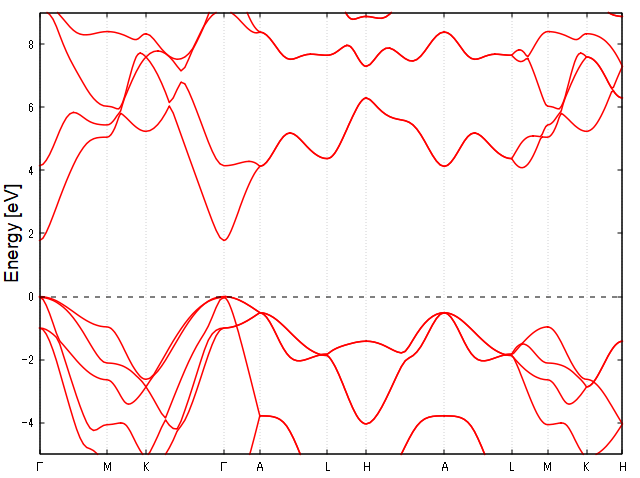
\includegraphics[scale=0.5]{./chap03/GaN_band.png}
  \caption{gnuplotで作成したバンド分散図}
  \label{fig_gnuplot}
\end{figure}
gnuplotのほうが入力パラメータは多いが、グラフの自由度は高い。
また、pltファイルを一度作成すれば、使いまわすことができるので、
二回目以降はそれほど手間がかからないこともメリットである。

\subsection{k点パス}
